\chapter{CFDDB测试集的建立}
\label{chap:establishCFDDB}

在选择正确的算法之前,我们应当选择或者建立一套测试集,以检测算法执行的效果。在人脸检测和识别的领域,已经有数量众多的公开数据集用于训练和测试,常见的有WiderFace[4],FDDB[5],LFW[6]等等。然而这些数据集中的人脸大多是欧美人,而且每张照片中的人脸数量也有限,如\ref{fig:chap1:picfromwider}。而如\ref{fig:chap1:picfromcfddb} 所示我们从监控录像中提取的图片亚洲人偏多,人脸往往是模糊的,大角度的,或是被遮挡的。因此,现有的测试集无法满足我们的测试需求,根据这个需要我们建立了自己的测试集CFDDB。

\begin{figure}[!htp]
	\centering
	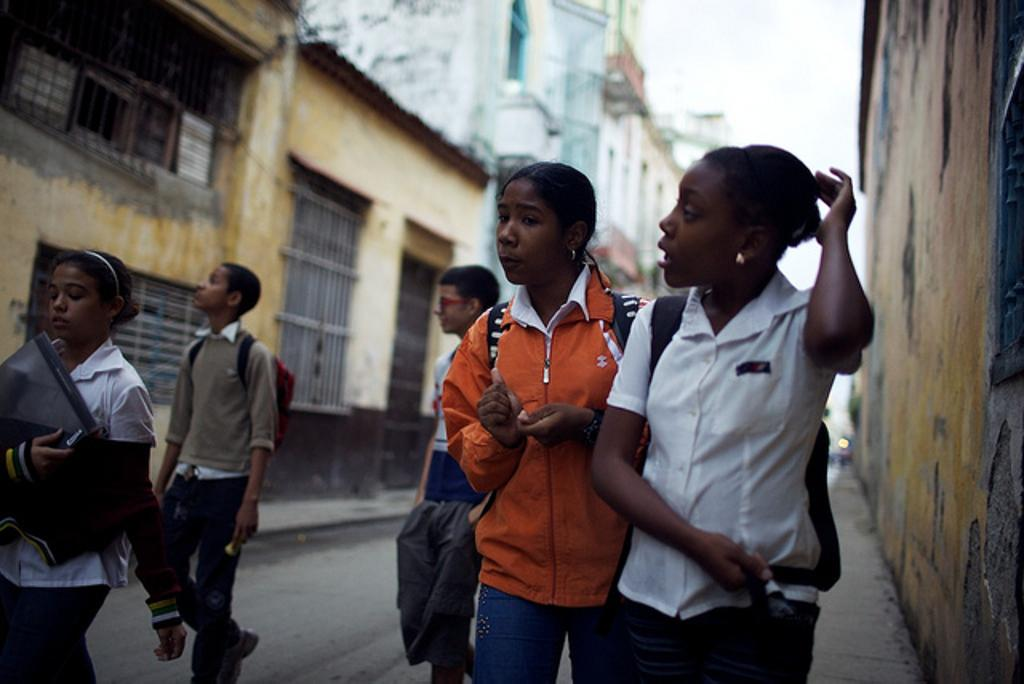
\includegraphics[height=6cm]{chap1/1.jpg}
	\bicaption{WiderFace 测试集中的一张图片}{A picture from WiderFace}
	\label{fig:chap1:picfromwider}
\end{figure}

\begin{figure}[!htp]
	\centering
	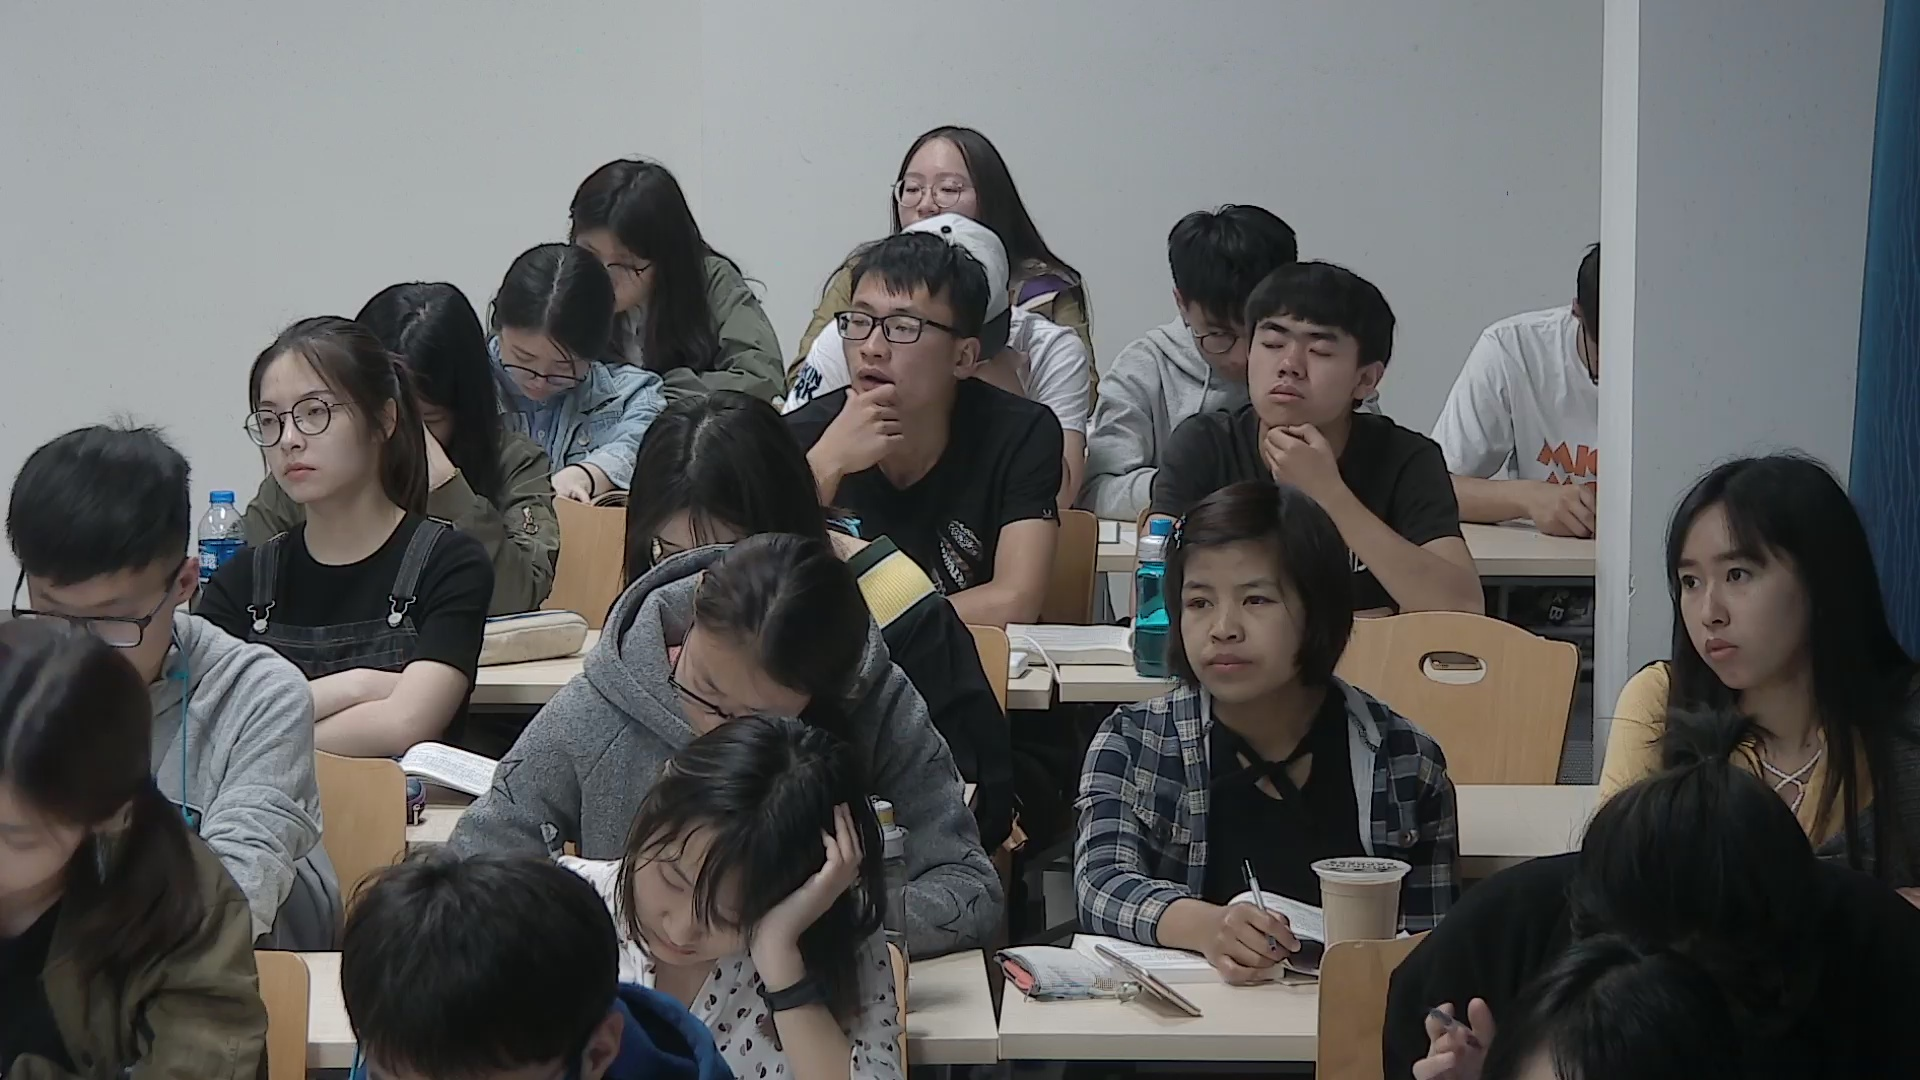
\includegraphics[height=6cm]{chap1/2.jpg}
	\bicaption{CFDDB 测试集中的一张图片}{A picture from CFDDB}
	\label{fig:chap1:picfromcfddb}
\end{figure}


\section{CFDDB测试集图片标注规则}

测试集图片由从一段15分钟的监控录像中每隔100帧截取一帧产生,共有149张图片。标注人需要标注一张图片中使用矩形框标注全部可识别人脸。标注的矩形框应当以人脸的鼻子为中心,矩形框区域面积应当大概是人脸区域面积的两倍。\ref{fig:chap1:cfddblbexp}为CFDDB中一张图片的标注可视化之后的效果,其中,绿色的矩形框为标注人标注的人脸区域。

\begin{figure}[!htp]
	\centering
	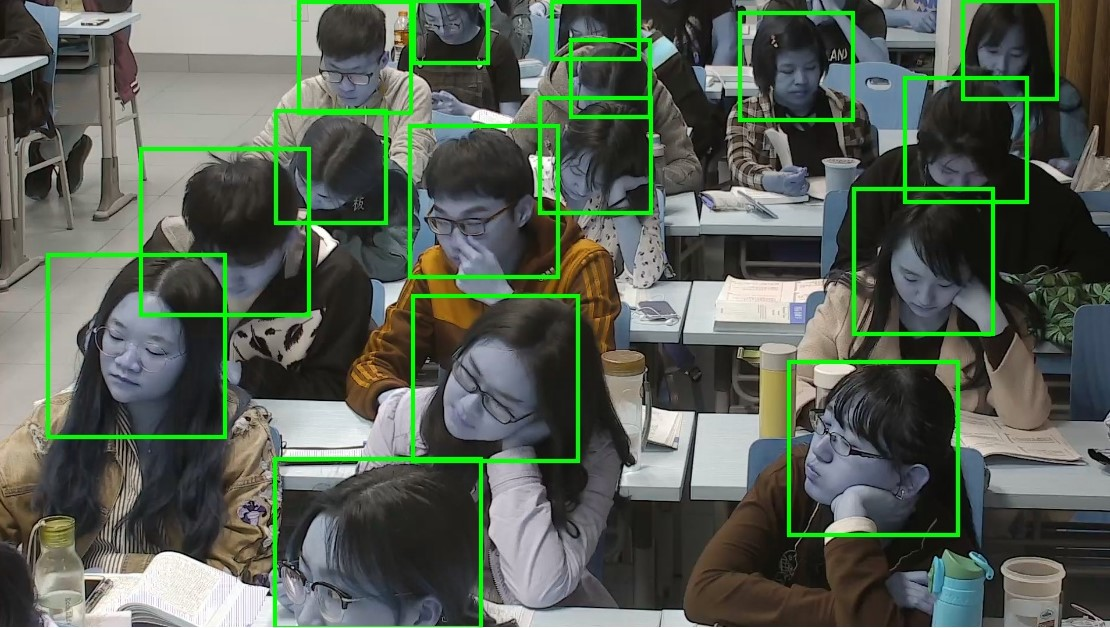
\includegraphics[height=6cm]{chap1/3.jpg}
	\bicaption{CFDDB 标注示例}{A lable example from CFDDB}
	\label{fig:chap1:cfddblbexp}
\end{figure}

矩形框标注完毕之后需要给每一个矩形框添加一个标签,这个标签是标注人脸的全局名称。标签添加完毕之后,将一张图片中所有矩形框的位置信息和标签信息写入与图片相同名字的XML文件进行保存。

\section{CFDDB测试集的纠错与预处理}

测试集的标注是人为进行的,有可能会出现差错,所以在将标注信息加入测试集之前,还需要对标注的信息进行认真反复的比对,确保标注信息的正确性。在本次比对中,共发现六处错误。修改所有错误之后,测试集中共有可用图片134张,人脸1087个,总人数84人。

测试集的预处理分为四步。第一步是将所有人脸图像区域切割出来,并将相同的人脸放到以该人脸的标签为名的文件夹下。这么做的目的是方便建立之后的识别数据库,而且通过对每个文件夹中的内容的比对,可以再次检验人为标注是否准确。

第二步是对齐所有人脸。由于人为标注的人脸有大有小,所以需要将所有截出的人脸图像对齐到相同大小。CFDDB在建立时保持了原有人脸的长宽比,不足的地方以空白图像补全,之后使用线性插值的方式将所有人脸缩放到了长150像素,宽150像素的大小。

第三步是将所有对齐的人脸进行预识别,得到特征向量。CFDDB在建立时使用了MTCNN[7]进行校正,使用ArcFace算法[2]进行校正后提取特征向量的过程。最后,每一张截出的人脸图像都转化为了一个128维的特征向量。

最后一步是对所有抽取出的特征向量进行聚类,使用\ref{algo:classcenter}计算出每个类的类中心作为该人脸的标准特征向量保存到以该人脸标签为文件名的Numpy向量文件中。

\begin{algorithm}
	% \begin{algorithm}[H] % 强制定位
	\caption{求类中心}
	\label{algo:classcenter}
	\begin{algorithmic}[1] %每行显示行号
		\Require $Array$类成员向量数组,$n$类成员个数 % 输入
		\Ensure $center$类中心向量 % 输出
		\Function {CalcAverage}{$Array, n$}
		\State $result \gets 0$
		\For {$i = 0 \to n-1$}
		\State $result \gets result + Array[i]$
		\EndFor
		\State \Return{$result$}
		\EndFunction
		\State %空一行
		\Function{Normalize}{$vector$}
		\State $l\gets 128$
		\State $norm\gets 0$
		\For {$j = 0 \to l-1$}
		\State $norm\gets norm + vector[j] * vector[j]$
		\EndFor
		\State $norm\gets \sqrt{norm}$
		\State $norm\gets vector / norm$
		\State \Return{$norm$}
		\EndFunction
		\State
		\Function{CalcCenter}{$Array, n$}
		\State $center\gets $\Call{ClacAverage}{$Array, n$}
		\State $center\gets $\Call{Normalize}{$center$}
		\State \Return{$centor$}
		\EndFunction
	\end{algorithmic}
\end{algorithm}

\section{CFDDB测试集的使用}

CFDDB测试集既可以用来测试无感知人脸检测算法的准确性,又可以测试无感知人脸识别算法的准确性。CFDDB中的所有内容都可以在CFDDB的Github主页[8]中找到,主页中还包含了针对不同算法检测的示例程序。下面我们分别介绍如何使用CFDDB数据集:

\subsection{使用CFDDB测试人脸检测算法}

下述检测方法中$ImageList$表示CFDDB测试集的图像列表,$GroundTruth[image]$表示对应$image$图片的人为标注区域列表,$Detect[image]$表示对应$image$图片使用人脸检测算法得到的区域列表,$TargetIOU$表示人为设定的标定区域和检测区域的交叠率。检测方法如下:

\begin{enumerate}
	\item 从$ImageList$中取出待检测的图像$image$。
	\item 调用待测的检测算法得到$Detect[image]$,同时读出人为标注信息$GroundTruth[image]$。
	\item 计算$Detect[image]$中每一项与$GroundTruth[image]$中每一项的交叠率,如果最大的交叠率超过了预设的$TargetIOU$则认为成功的检测到了一张人脸。
	\item 计算所有检测到的人脸数目,并将检测错误的信息输出分析检测算法存在的缺陷。
\end{enumerate}

\subsection{使用CFDDB测试人脸识别算法}

下述检测方法中$FaceImage$表示待检测的人脸图片区域,$GroundTruth[FaceImage]$表示人为标注的人脸编号,$Recognize[FaceImage]$表示识别得出的人脸向量,$FaceList$表示经过预处理后得到的每一个人脸编号对应的类中心向量。检测方法如下:

\begin{enumerate}
	\item 取出待检测人脸区域的人为标注编号$GroundTruth[FaceImage]$。
	\item 调用人脸识别算法得到$Recognize[FaceImage]$。
	\item 计算$Recognize[FaceImage]$到$FaceList$中每一项的欧氏距离,将距离最小的一项对应的标签与$GroundTruth[FaceImage]$比对,如果相同,认为识别正确;如果不同,认为识别错误。
	\item 计算所有识别正确的人脸数目,并将错误信息输出分析识别算法存在的缺陷。
\end{enumerate}


